\documentclass[11pt,a4paper]{article}

% Modern packages
\usepackage[utf8]{inputenc}
\usepackage[T1]{fontenc}
\usepackage{lmodern}
\usepackage[margin=1in]{geometry}
\usepackage{hyperref}
\usepackage{xcolor}
\usepackage{booktabs}
\usepackage{listings}
\usepackage{graphicx}
\usepackage{amsmath}
\usepackage{natbib}
\usepackage{tikz}
\usetikzlibrary{shapes.geometric, arrows.meta, positioning, fit, backgrounds}

% Colors
\definecolor{codegreen}{rgb}{0,0.6,0}
\definecolor{codegray}{rgb}{0.5,0.5,0.5}
\definecolor{codepurple}{rgb}{0.58,0,0.82}
\definecolor{backcolour}{rgb}{0.97,0.97,0.97}
\definecolor{linkblue}{rgb}{0.0,0.4,0.7}

% Hyperref setup
\hypersetup{
    colorlinks=true,
    linkcolor=linkblue,
    citecolor=linkblue,
    urlcolor=linkblue
}

% Code listing style
\lstdefinestyle{rustcode}{
    backgroundcolor=\color{backcolour},
    commentstyle=\color{codegreen},
    keywordstyle=\color{codepurple}\bfseries,
    numberstyle=\tiny\color{codegray},
    stringstyle=\color{codegreen},
    basicstyle=\ttfamily\small,
    breakatwhitespace=false,
    breaklines=true,
    captionpos=b,
    keepspaces=true,
    numbers=none,
    showspaces=false,
    showstringspaces=false,
    showtabs=false,
    tabsize=2,
    frame=single,
    framerule=0.5pt,
    rulecolor=\color{codegray}
}

\lstset{style=rustcode}

% Title
\title{\textbf{PDBRust: A High-Performance Rust Library for Protein Structure File Parsing and Analysis}}

\author{Hosein Fooladi\\
\small University of Vienna, Austria\\
\small \texttt{hosein.fooladi@univie.ac.at}\\
\small ORCID: \href{https://orcid.org/0000-0002-3124-2761}{0000-0002-3124-2761}}

\date{}

\begin{document}

\maketitle

\begin{abstract}
We present PDBRust, an open-source Rust library for parsing and analyzing Protein Data Bank (PDB) and mmCIF structure files. PDBRust provides a unified interface for both file formats with automatic format detection, native gzip decompression, comprehensive structural analysis capabilities, and seamless integration with the RCSB PDB database. Benchmarks demonstrate 40--260$\times$ speedups compared to equivalent Python implementations for common operations. The library has been validated against the entire PDB archive (230,655 structures) with a 100\% success rate and zero parsing failures, demonstrating production-ready robustness. PDBRust is designed for high-throughput structural bioinformatics pipelines and machine learning applications requiring efficient processing of large protein structure datasets. PDBRust is available at \url{https://github.com/HFooladi/pdbrust} and through the Rust package registry at \url{https://crates.io/crates/pdbrust}.
\end{abstract}

\begin{figure}[h]
\centering
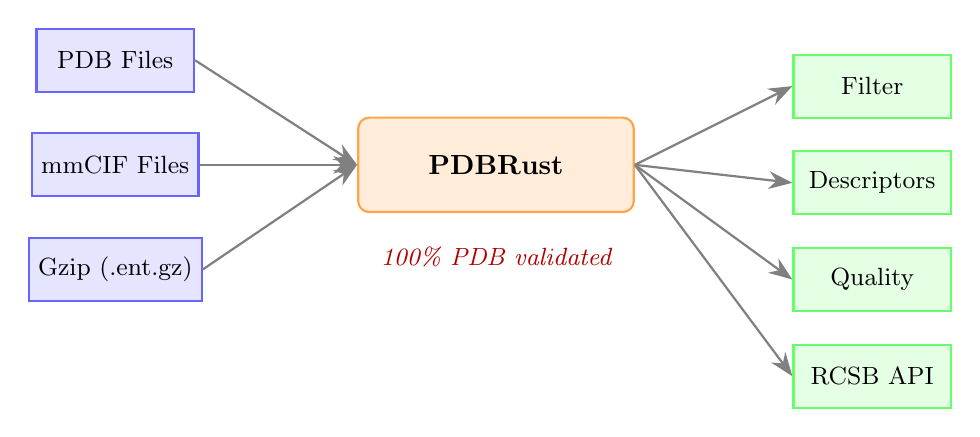
\begin{tikzpicture}[
    node distance=1.5cm,
    inputbox/.style={rectangle, draw=blue!60, fill=blue!10, thick, minimum width=2cm, minimum height=0.8cm, font=\small},
    corebox/.style={rectangle, draw=orange!70, fill=orange!15, thick, rounded corners, minimum width=3.5cm, minimum height=1.2cm, font=\bfseries},
    outputbox/.style={rectangle, draw=green!60, fill=green!10, thick, minimum width=2cm, minimum height=0.8cm, font=\small},
    arrow/.style={-{Stealth[length=3mm]}, thick, gray}
]

% Input nodes
\node[inputbox] (pdb) {PDB Files};
\node[inputbox, below=0.5cm of pdb] (mmcif) {mmCIF Files};
\node[inputbox, below=0.5cm of mmcif] (gzip) {Gzip (.ent.gz)};

% Core processor
\node[corebox, right=2cm of mmcif] (core) {PDBRust};

% Output nodes
\node[outputbox, right=2cm of core, yshift=1cm] (filter) {Filter};
\node[outputbox, below=0.4cm of filter] (desc) {Descriptors};
\node[outputbox, below=0.4cm of desc] (quality) {Quality};
\node[outputbox, below=0.4cm of quality] (rcsb) {RCSB API};

% Arrows
\draw[arrow] (pdb.east) -- (core.west);
\draw[arrow] (mmcif.east) -- (core.west);
\draw[arrow] (gzip.east) -- (core.west);
\draw[arrow] (core.east) -- (filter.west);
\draw[arrow] (core.east) -- (desc.west);
\draw[arrow] (core.east) -- (quality.west);
\draw[arrow] (core.east) -- (rcsb.west);

% Performance label
\node[below=0.3cm of core, font=\small\itshape, text=red!70!black] {100\% PDB validated};

\end{tikzpicture}
\caption{PDBRust architecture: unified parsing of PDB/mmCIF files with modular analysis features.}
\label{fig:graphical-abstract}
\end{figure}

\section{Introduction}

Protein structure analysis is fundamental to computational biology, drug discovery, and machine learning applications in structural bioinformatics. The Protein Data Bank (PDB) \cite{berman2000protein} contains over 200,000 experimentally determined structures, with data available in both the legacy PDB format and the modern mmCIF format. Processing these structures efficiently is essential for large-scale analyses, yet existing tools often sacrifice performance for ease of use.

Python libraries such as Biopython \cite{cock2009biopython} and MDAnalysis \cite{michaud2011mdanalysis} provide comprehensive functionality but face inherent performance limitations due to interpreter overhead and memory management. For applications requiring processing of thousands of structures---such as training machine learning models on structural data or genome-wide structural analysis---these limitations become significant bottlenecks.

We developed PDBRust to address this gap, providing a Rust library that combines the safety and performance characteristics of systems programming with an ergonomic API suitable for scientific computing. Rust's zero-cost abstractions, memory safety guarantees, and lack of garbage collection overhead make it well-suited for computationally intensive structural biology applications.

\section{Features and Implementation}

\subsection{Core Parsing}

PDBRust supports both PDB and mmCIF file formats through a unified \texttt{PdbStructure} data model. The parser automatically detects file format based on content and handles:

\begin{itemize}
    \item ATOM/HETATM coordinate records with full metadata
    \item SEQRES sequence information
    \item SSBOND disulfide bond definitions
    \item CONECT connectivity records
    \item Multi-model structures (NMR ensembles)
    \item Alternate conformations (altlocs)
\end{itemize}

\subsection{Modular Feature System}

PDBRust employs Rust's feature flag system to provide optional functionality while keeping the core library lightweight. Available modules include:

\begin{itemize}
    \item \textbf{filter}: Structure filtering, chain extraction, ligand removal, and coordinate transformations
    \item \textbf{descriptors}: Structural metrics including radius of gyration, amino acid composition, and geometric properties
    \item \textbf{quality}: Structure quality assessment for analysis readiness
    \item \textbf{rcsb}: Direct integration with RCSB PDB search API and file download
\end{itemize}

\subsection{API Design}

The library provides a fluent API for method chaining, enabling concise expression of complex operations:

\begin{lstlisting}[language=Python,caption={Example: Structure cleaning and analysis}]
let structure = parse_pdb_file("protein.pdb")?;

// Fluent API for structure manipulation
let cleaned = structure
    .remove_ligands()
    .keep_only_chain("A")
    .keep_only_backbone();

// Compute structural descriptors
let rg = cleaned.radius_of_gyration();
let composition = cleaned.aa_composition();
\end{lstlisting}

\section{Performance}

We benchmarked PDBRust against equivalent Python implementations using the \texttt{libraryPDB} package on a representative protein structure (PDB: 1A2B, 4,728 atoms). Table~\ref{tab:benchmarks} summarizes the results.

\begin{table}[h]
\centering
\caption{Performance comparison between PDBRust and Python (libraryPDB)}
\label{tab:benchmarks}
\begin{tabular}{lccc}
\toprule
\textbf{Operation} & \textbf{Python (ms)} & \textbf{Rust (ms)} & \textbf{Speedup} \\
\midrule
Parse PDB file & 15.2 & 0.36 & 42$\times$ \\
Remove ligands & 8.0 & 0.03 & 267$\times$ \\
Get CA coordinates & 7.2 & 0.03 & 240$\times$ \\
Radius of gyration & 2.0 & 0.05 & 40$\times$ \\
Max CA distance & 70.4 & 0.27 & 261$\times$ \\
\bottomrule
\end{tabular}
\end{table}

The substantial speedups (40--260$\times$) arise from several factors: (1) PDBRust parses the structure once and reuses it across operations, whereas Python libraries often re-parse for each call; (2) Rust's zero-cost abstractions eliminate runtime overhead; (3) efficient memory layout improves CPU cache utilization for coordinate-heavy operations.

\subsection{Full PDB Archive Validation}

To validate robustness and correctness, we benchmarked PDBRust against the entire Protein Data Bank archive comprising 230,655 gzip-compressed structure files. The library includes native gzip decompression support (via the \texttt{flate2} crate) for seamless processing of PDB archive distributions. Table~\ref{tab:pdb-validation} summarizes the results.

\begin{table}[h]
\centering
\caption{Full PDB archive validation results (230,655 structures)}
\label{tab:pdb-validation}
\begin{tabular}{lc}
\toprule
\textbf{Metric} & \textbf{Value} \\
\midrule
Total Structures & 230,655 \\
Success Rate & 100\% \\
Failed Parses & 0 \\
Total Atoms Parsed & 2,057,302,767 \\
Total Residues Parsed & 246,469,962 \\
Average Atoms/Structure & 8,919 \\
Processing Rate & $\sim$92 files/sec \\
Largest Structure & 2ku2 (1,290,100 atoms) \\
Smallest Structure & 5zmz (31 atoms) \\
\bottomrule
\end{tabular}
\end{table}

The 100\% success rate across all 230,655 structures demonstrates PDBRust's production-ready robustness for large-scale structural bioinformatics applications.

\section{Use Cases}

PDBRust is designed for:

\begin{itemize}
    \item \textbf{Machine learning pipelines}: Efficient feature extraction from large structure datasets for training geometric deep learning models
    \item \textbf{High-throughput screening}: Rapid processing of structure libraries for virtual screening campaigns
    \item \textbf{Structural bioinformatics}: Genome-wide analysis of protein structures and structure-function relationships
    \item \textbf{Web services}: Backend processing for structure analysis web applications requiring low latency
\end{itemize}

\section{Availability}

PDBRust is open-source software released under the MIT license. The source code is available at \url{https://github.com/HFooladi/pdbrust}. The library can be installed via the Rust package manager:

\begin{lstlisting}[language=bash]
cargo add pdbrust --features "filter,descriptors,rcsb"
\end{lstlisting}

Documentation is available at \url{https://docs.rs/pdbrust}.

\section{Conclusion}

PDBRust provides a high-performance, memory-safe library for protein structure file parsing and analysis. By leveraging Rust's systems programming capabilities, it achieves 40--260$\times$ speedups over Python alternatives while maintaining an ergonomic API. The library has been rigorously validated against the entire Protein Data Bank archive (230,655 structures) with a 100\% success rate, demonstrating production-ready robustness. The modular design allows users to include only the functionality they need, native gzip support enables direct processing of PDB archive distributions, and the RCSB integration enables seamless access to the Protein Data Bank. PDBRust is suitable for large-scale structural bioinformatics applications where performance and reliability are critical.

\section*{Acknowledgments}

We thank the Rust and structural biology communities for valuable feedback during development.

\bibliographystyle{unsrtnat}
\bibliography{reference}

\end{document}
